\documentclass[12pt,twoside,letterpaper]{article}
%NOTE: This report format is 

\usepackage{lipsum}
\usepackage{gensymb}
\newcommand{\reporttitle}{Modeling the Flight of a Frisbee}
\newcommand{\reportauthorOne}{Steven Ha}
\newcommand{\cidOne}{}
\newcommand{\reportauthorTwo}{Brendan Johnston}
\newcommand{\cidTwo}{}
\newcommand{\reportauthorThree}{Niel Mistry}
\newcommand{\cidThree}{}
\newcommand{\reporttype}{Coursework}
\bibliographystyle{unsrt}


% include files that load packages and define macros
%%%%%%%%%%%%%%%%%%%%%%%%%%%%%%%%%%%%%%%%%
% University Assignment Title Page 
% LaTeX Template
% Version 1.0 (27/12/12)
%
% This template has been downloaded from:
% http://www.LaTeXTemplates.com
%
% Original author:
% WikiBooks (http://en.wikibooks.org/wiki/LaTeX/Title_Creation)
%
% License:
% CC BY-NC-SA 3.0 (http://creativecommons.org/licenses/by-nc-sa/3.0/)
% 
% Instructions for using this template:
% This title page is capable of being compiled as is. This is not useful for 
% including it in another document. To do this, you have two options: 
%
% 1) Copy/paste everything between \begin{document} and \end{document} 
% starting at \begin{titlepage} and paste this into another LaTeX file where you 
% want your title page.
% OR
% 2) Remove everything outside the \begin{titlepage} and \end{titlepage} and 
% move this file to the same directory as the LaTeX file you wish to add it to. 
% Then add \input{./title_page_1.tex} to your LaTeX file where you want your
% title page.
%
%----------------------------------------------------------------------------------------
%	PACKAGES AND OTHER DOCUMENT CONFIGURATIONS
%----------------------------------------------------------------------------------------
\usepackage{ifxetex}
\usepackage{textpos}
\usepackage{natbib}
\usepackage{kpfonts}
\usepackage[letterpaper,hmargin=2.8cm,vmargin=2.0cm,includeheadfoot]{geometry}
\usepackage{ifxetex}
\usepackage{stackengine}
\usepackage{tabularx,longtable,multirow,subfigure,caption}%hangcaption
\usepackage{fncylab} %formatting of labels
\usepackage{fancyhdr}
\usepackage{color}
\usepackage[tight,ugly]{units}
\usepackage{url}
\usepackage{float}
\usepackage[english]{babel}
\usepackage{amsmath}
\usepackage{graphicx}
\usepackage[colorinlistoftodos]{todonotes}
\usepackage{dsfont}
\usepackage{epstopdf} % automatically replace .eps with .pdf in graphics
\usepackage{natbib}
\usepackage{backref}
\usepackage{array}
\usepackage{latexsym}
\usepackage{etoolbox}
\usepackage{listings}
\usepackage{color} %red, green, blue, yellow, cyan, magenta, black, white
\definecolor{mygreen}{RGB}{28,172,0} % color values Red, Green, Blue
\definecolor{mylilas}{RGB}{170,55,241}
\usepackage[numbib]{tocbibind}
\usepackage{mathtools}
\newcommand{\vectorproj}[2][]{\textit{proj}_{\vect{#1}}\vect{#2}}
\usepackage{setspace}
\usepackage{multicol}

\lstset{language=Matlab,%
    %basicstyle=\color{red},
    breaklines=true,%
    morekeywords={matlab2tikz},
    keywordstyle=\color{blue},%
    morekeywords=[2]{1}, keywordstyle=[2]{\color{black}},
    identifierstyle=\color{black},%
    stringstyle=\color{mylilas},
    commentstyle=\color{mygreen},%
    showstringspaces=false,%without this there will be a symbol in the places where there is a space
    numbers=left,%
    numberstyle={\tiny \color{black}},% size of the numbers
    numbersep=9pt, % this defines how far the numbers are from the text
    emph=[1]{for,end,break},emphstyle=[1]\color{red}, %some words to emphasise
    %emph=[2]{word1,word2}, emphstyle=[2]{style},    
}

\usepackage{enumerate} % for numbering with [a)] format 



\ifxetex
\usepackage{fontspec}
\setmainfont[Scale=.8]{OpenDyslexic-Regular}
\else
\usepackage[pdftex,pagebackref,hypertexnames=false,colorlinks]{hyperref} % provide links in pdf
\hypersetup{pdftitle={},
  pdfsubject={}, 
  pdfauthor={\reportauthorOne},
  pdfkeywords={}, 
  pdfstartview=FitH,
  pdfpagemode={UseOutlines},% None, FullScreen, UseOutlines
  bookmarksnumbered=true, bookmarksopen=true, colorlinks,
    citecolor=black,%
    filecolor=black,%
    linkcolor=black,%
    urlcolor=black}
\usepackage[all]{hypcap}
\fi

\usepackage{tcolorbox}

% various theorems
\usepackage{ntheorem}
\theoremstyle{break}
\newtheorem{lemma}{Lemma}
\newtheorem{theorem}{Theorem}
\newtheorem{remark}{Remark}
\newtheorem{definition}{Definition}
\newtheorem{proof}{Proof}

% example-environment
\newenvironment{example}[1][]
{ 
\vspace{4mm}
\noindent\makebox[\linewidth]{\rule{\hsize}{1.5pt}}
\textbf{Example #1}\\
}
{ 
\noindent\newline\makebox[\linewidth]{\rule{\hsize}{1.0pt}}
}



%\renewcommand{\rmdefault}{pplx} % Palatino
% \renewcommand{\rmdefault}{put} % Utopia

\ifxetex
\else
\renewcommand*{\rmdefault}{bch} % Charter
\renewcommand*{\ttdefault}{cmtt} % Computer Modern Typewriter
%\renewcommand*{\rmdefault}{phv} % Helvetica
%\renewcommand*{\rmdefault}{iwona} % Avant Garde
\fi

\setlength{\parindent}{0em}  % indentation of paragraph

\setlength{\headheight}{14.5pt}
\pagestyle{fancy}
\fancyfoot[ER,OL]{\thepage}%Page no. in the left on
                                %odd pages and on right on even pages
\fancyfoot[OC,EC]{\sffamily }
\renewcommand{\headrulewidth}{0.1pt}
\renewcommand{\footrulewidth}{0.1pt}
\captionsetup{margin=10pt,font=small,labelfont=bf}


%--- chapter heading

\def\@makechapterhead#1{%
  \vspace*{10\p@}%
  {\parindent \z@ \raggedright %\sffamily
        %{\Large \MakeUppercase{\@chapapp} \space \thechapter}
        %\\
        %\hrulefill
        %\par\nobreak
        %\vskip 10\p@
    \interlinepenalty\@M
    \Huge \bfseries 
    \thechapter \space\space #1\par\nobreak
    \vskip 30\p@
  }}

%---chapter heading for \chapter*  
\def\@makeschapterhead#1{%
  \vspace*{10\p@}%
  {\parindent \z@ \raggedright
    \sffamily
    \interlinepenalty\@M
    \Huge \bfseries  
    #1\par\nobreak
    \vskip 30\p@
  }}
  



% %%%%%%%%%%%%% boxit
\def\Beginboxit
   {\par
    \vbox\bgroup
	   \hrule
	   \hbox\bgroup
		  \vrule \kern1.2pt %
		  \vbox\bgroup\kern1.2pt
   }

\def\Endboxit{%
			      \kern1.2pt
		       \egroup
		  \kern1.2pt\vrule
		\egroup
	   \hrule
	 \egroup
   }	

\newenvironment{boxit}{\Beginboxit}{\Endboxit}
\newenvironment{boxit*}{\Beginboxit\hbox to\hsize{}}{\Endboxit}



\allowdisplaybreaks

\makeatletter
\newcounter{elimination@steps}
\newcolumntype{R}[1]{>{\raggedleft\arraybackslash$}p{#1}<{$}}
\def\elimination@num@rights{}
\def\elimination@num@variables{}
\def\elimination@col@width{}
\newenvironment{elimination}[4][0]
{
    \setcounter{elimination@steps}{0}
    \def\elimination@num@rights{#1}
    \def\elimination@num@variables{#2}
    \def\elimination@col@width{#3}
    \renewcommand{\arraystretch}{#4}
    \start@align\@ne\st@rredtrue\m@ne
}
{
    \endalign
    \ignorespacesafterend
}
\newcommand{\eliminationstep}[2]
{
    \ifnum\value{elimination@steps}>0\leadsto\quad\fi
    \left[
        \ifnum\elimination@num@rights>0
            \begin{array}
            {@{}*{\elimination@num@variables}{R{\elimination@col@width}}
            |@{}*{\elimination@num@rights}{R{\elimination@col@width}}}
        \else
            \begin{array}
            {@{}*{\elimination@num@variables}{R{\elimination@col@width}}}
        \fi
            #1
        \end{array}
    \right]
    & 
    \begin{array}{l}
        #2
    \end{array}
    &%                                    moved second & here
    \addtocounter{elimination@steps}{1}
}
\makeatother

%% Fast macro for column vectors
\makeatletter  
\def\colvec#1{\expandafter\colvec@i#1,,,,,,,,,\@nil}
\def\colvec@i#1,#2,#3,#4,#5,#6,#7,#8,#9\@nil{% 
  \ifx$#2$ \begin{bmatrix}#1\end{bmatrix} \else
    \ifx$#3$ \begin{bmatrix}#1\\#2\end{bmatrix} \else
      \ifx$#4$ \begin{bmatrix}#1\\#2\\#3\end{bmatrix}\else
        \ifx$#5$ \begin{bmatrix}#1\\#2\\#3\\#4\end{bmatrix}\else
          \ifx$#6$ \begin{bmatrix}#1\\#2\\#3\\#4\\#5\end{bmatrix}\else
            \ifx$#7$ \begin{bmatrix}#1\\#2\\#3\\#4\\#5\\#6\end{bmatrix}\else
              \ifx$#8$ \begin{bmatrix}#1\\#2\\#3\\#4\\#5\\#6\\#7\end{bmatrix}\else
                 \PackageError{Column Vector}{The vector you tried to write is too big, use bmatrix instead}{Try using the bmatrix environment}
              \fi
            \fi
          \fi
        \fi
      \fi
    \fi
  \fi 
}  
\makeatother

\robustify{\colvec}

%%% Local Variables: 
%%% mode: latex
%%% TeX-master: "notes"
%%% End: 
 % various packages needed for maths etc.
% quick way of adding a figure
\newcommand{\fig}[3]{
 \begin{center}
 \scalebox{#3}{\includegraphics[#2]{#1}}
 \end{center}
}

%\newcommand*{\point}[1]{\vec{\mkern0mu#1}}
\newcommand{\ci}[0]{\perp\!\!\!\!\!\perp} % conditional independence
\newcommand{\point}[1]{{#1}} % points 
%\renewcommand{\vec}[1]{{\boldsymbol{{#1}}}} % vector
\newcommand{\mat}[1]{{\boldsymbol{{#1}}}} % matrix
\newcommand{\R}[0]{\mathds{R}} % real numbers
\newcommand{\Z}[0]{\mathds{Z}} % integers
\newcommand{\N}[0]{\mathds{N}} % natural numbers
\newcommand{\nat}[0]{\mathds{N}} % natural numbers
\newcommand{\Q}[0]{\mathds{Q}} % rational numbers
\ifxetex
\newcommand{\C}[0]{\mathds{C}} % complex numbers
\else
\newcommand{\C}[0]{\mathds{C}} % complex numbers
\fi
\newcommand{\tr}[0]{\text{tr}} % trace
\renewcommand{\d}[0]{\mathrm{d}} % total derivative
\newcommand{\inv}{^{-1}} % inverse
\newcommand{\id}{\mathrm{id}} % identity mapping
\renewcommand{\dim}{\mathrm{dim}} % dimension
\newcommand{\rank}[0]{\mathrm{rk}} % rank
\newcommand{\determ}[1]{\mathrm{det}(#1)} % determinant
\newcommand{\scp}[2]{\langle #1 , #2 \rangle}
\newcommand{\kernel}[0]{\mathrm{ker}} % kernel/nullspace
\newcommand{\img}[0]{\mathrm{Im}} % image
\newcommand{\idx}[1]{{(#1)}}
\DeclareMathOperator*{\diag}{diag}
\newcommand{\E}{\mathds{E}} % expectation
\newcommand{\var}{\mathds{V}} % variance
\newcommand{\gauss}[2]{\mathcal{N}\big(#1,\,#2\big)} % gaussian distribution N(.,.)
\newcommand{\gaussx}[3]{\mathcal{N}\big(#1\,|\,#2,\,#3\big)} % gaussian distribution N(.|.,.)
\newcommand{\gaussBig}[2]{\mathcal{N}\left(#1,\,#2\right)} % see above, but with brackets that adjust to the height of the arguments
\newcommand{\gaussxBig}[3]{\mathcal{N}\left(#1\,|\,#2,\,#3\right)} % see above, but with brackets that adjust to the height of the arguments
\DeclareMathOperator{\cov}{Cov} % covariance (matrix) 
\ifxetex
\renewcommand{\T}[0]{^\top} % transpose
\else
\newcommand{\T}[0]{^\top}
\fi
% matrix determinant
\newcommand{\matdet}[1]{
\left|
\begin{matrix}
#1
\end{matrix}
\right|
}



%%% various color definitions
\definecolor{darkgreen}{rgb}{0,0.6,0}

\newcommand{\blue}[1]{{\color{blue}#1}}
\newcommand{\red}[1]{{\color{red}#1}}
\newcommand{\green}[1]{{\color{darkgreen}#1}}
\newcommand{\orange}[1]{{\color{orange}#1}}
\newcommand{\magenta}[1]{{\color{magenta}#1}}
\newcommand{\cyan}[1]{{\color{cyan}#1}}


% redefine emph
\renewcommand{\emph}[1]{\blue{\bf{#1}}}

% place a colored box around a character
\gdef\colchar#1#2{%
  \tikz[baseline]{%
  \node[anchor=base,inner sep=2pt,outer sep=0pt,fill = #2!20] {#1};
    }%
}%
 % short-hand notation and macros

%%%%%%%%%%%%%%%%%%%%%%%%%%%%

\begin{document}
% front page
% Last modification: 2016-09-29 (Marc Deisenroth)
% Modification for UW: 2017-05-22 (jphickey)
% Modification for UW: 2017-10-30 (jphickey)
\begin{titlepage}

\newcommand{\HRule}{\rule{\linewidth}{0.5mm}} % Defines a new command for the horizontal lines, change thickness here


%----------------------------------------------------------------------------------------
%	LOGO SECTION
%----------------------------------------------------------------------------------------



\begin{center} % Center remainder of the page

%----------------------------------------------------------------------------------------
%	HEADING SECTIONS
%----------------------------------------------------------------------------------------


\includegraphics[width = 10cm]{./figures/uw}\\[1.5cm] 
\textbf{\textsc{\Large MTE202 - Ordinary Differential Equations}}\\[1.0cm] 
\textsc{\Large University of Waterloo}\\[0.5cm] 
\textsc{\large Department of Mechanical and Mechatronics Engineering}\\[0.95cm] 

%----------------------------------------------------------------------------------------
%	TITLE SECTION
%----------------------------------------------------------------------------------------

\HRule \\[0.4cm]
{ \huge \bfseries \reporttitle}\\ % Title of your document
\HRule \\[1.5cm]
\end{center}
%----------------------------------------------------------------------------------------
%	AUTHOR SECTION
%----------------------------------------------------------------------------------------

%\begin{minipage}{0.4\hsize}
\vspace{1.5cm}
\begin{flushleft} \large
\textit{Authors:}\\
\reportauthorOne ~(ID: \cidOne) \\
\reportauthorTwo ~(ID: \cidTwo)\\   % Your name
\reportauthorThree ~(ID: \cidThree)
\end{flushleft}
\vspace{3.5cm}
\makeatletter
Date: \@date 

\vfill % Fill the rest of the page with whitespace



\makeatother


\end{titlepage}



%%%%%%%%%%%%%%%%%%%%%%%%%%%% table of contents
\tableofcontents
\newpage

%%%%%%%%%%%%%%%%%%%%%%%%%%%% list of figures
\listoffigures
\newpage


\section{Nomenclature}
{ \setstretch{2}
$\alpha = $ angle of attack (rad)\cite{Morrison2005}\\
$\alpha_0 = $ angle of attack that causes the least lift (rad)\cite{Baumback2010}\\
$A = $ area of Frisbee ($m^2$) \\
$ac = $ aerodynamic center\\
$C_D = $ coefficient of drag \cite{Morrison2005}\\
$C_D0 = $ form drag constant \cite{Baumback2010}\\ 
$C_D\alpha$ = induced drag constant \cite{Baumback2010}\\
$C_L = $ coefficient of lift \cite{Baumback2010}\\
$C_L0 = $ lift equation y-intercept \cite{Baumback2010}\\ 
$C_L\alpha = $ lift equation slope\\
$\vec{F}_D = $ drag force (N)\\
$\vec{F}_L = $ lift force (N)\\
$g = $ acceleration due to gravity m/$s^2$\\
$I_z = $ mass moment of inertia about z (kg$\cdot$m\textsuperscript{2})\\
$\eta = $ angle between aerodynamic center and x' (rad)\\
$M_0 = $ zero lift pitching moment (N$\cdot$m)\\ 
$\rho = $ density of air (kg$\cdot$m\textsuperscript{-3})\\
$\dot{p} = \text{pitching rate (rad/s)}$\\
$P = $  Pitching Moment (N$\cdot$m)\\
$\dot{r} = $ rolling rate (rad/s)\\
$R = $ Rolling Moment (N$\cdot$m)\\
$\vec{v} = $ velocity of Frisbee (m/s)\\
$x,y,z = $ unit vectors of reference frame of Frisbee parallel to global reference frame\\
$x',y',z' = $ unit vectors of reference frame of Frisbee which rotates with Frisbee\\
$X,Y,Z = $ unit vectors of the global inertial reference frame\\
}
\newpage

\begin{multicols}{2}
%%%%%%%%%%%%%%%%%%%%%%%%%%%% Main document

\section{Introduction}
\setlength{\parindent}{5ex}
The Frisbee is a popular recreational device with over 300  million units being sold since its introduction over 40 years ago \cite{Sheppard}. In sports such as Ultimate and Disc Golf, being able to predict the trajectory that is thrown is imperative to succeeding at the sport. Though this can be learned through practice , it is also possible to create a mathematical model to predict the trajectory of a Frisbee under certain conditions.\par
To understand this report, an understanding of the physics behind the flight of a Frisbee is needed. A Frisbee will experience lift, drag and gravity as it glides through the air. The lift force is produced by the pressure difference from air flowing over the top of the Frisbee faster than the air flowing the bottom of the Frisbee. Using the Bernoulli Principle a equation for the lift force can be derived \cite{Morrison2005}:


%Lift equation
\begin{equation}
\centering
F_{L} = \frac{1}{2}\rho v^2 A C_{L}
\label{eqLiftForce}
\end{equation}

It should be noted that the area in this equation does not change depending on the pitch of the Frisbee. In addition $C_{L}$ is a function of the angle of attack which is given below \eqref{eqCoeffLift}. The angle of attack is the angle between the plane of the Frisbee and the velocity vector. The constants in equation \eqref{eqCoeffLift} are determined based on the physical properties of the Frisbee ($C_L0 = 0.15$ and $C_L\alpha = 1.4$) \cite{Morrison2005}.

%Coefficient of lift equation
\begin{equation}
\centering
C_{L} = C_{L0} + C_{L\alpha} \alpha 
\label{eqCoeffLift}
\end{equation}

The drag relationship used to calculate drag force is dependent on the Reynolds number. For an average Frisbee throw and sea level conditions, the Reynolds number is $2.59\times 10^5$. This means that the Prandtl relationship for drag needs to be used \cite{Morrison2005}: 

%Drag force equation
\begin{equation}
\centering
F_{D} = -\frac{C_{D}\rho A v^2}{2} 
\label{eqDragForce}
\end{equation}

The coefficient of drag is also a function of the angle of attack which is defined below \cite{Morrison2005}.

%Drag coefficient equation
\begin{equation}
\centering
C_{D} = C_{D0} + C_{D\alpha} (\alpha-\alpha_{0})^2 
\label{eqCoeffDrag}
\end{equation}

All the constants in \eqref{eqCoeffDrag} depend on the physical property of the Frisbee with $C_{D0} = 0.08$, $C_{D\alpha} = 2.72$ and $\alpha_0 = -4\degree$ \cite{Morrison2005}\cite{Baumback2010}. The figure below summarizes the forces on a Frisbee.

\begin{figure}[H]
\centering
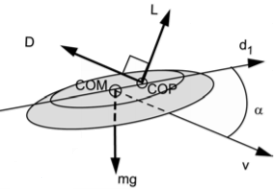
\includegraphics[width=4cm]{figures/Frisbee.PNG}
\caption{Lift and Drag acting on the CoP of a Frisbee \cite{HummelIdentificationData}}
\label{FrisbeeDiagram}
\end{figure}
In addition to the forces acting on the Frisbee, the flight of a Frisbee also depends on its rotation. The angular velocity in the Frisbee causes the gyroscopic effect which allows it to be very stable in the air. This means that it is resistant to the moments caused by the the lift and drag forces acting about the center of mass. These moments are due to the fact that the lift and drag forces act on a point called the center of pressure which is offset from the center of mass. These moments can be simply calculated by \cite{Morrison2005}:

%Moment equation
\begin{equation}
\centering
\vec{\tau} = \vec{r} \times \vec{F}  
\label{eqTorque}
\end{equation}

\vfill
\newpage
%%%%%%%%%%%%%%%%%%%%%%%%%%%%%%% Assumptions
\section{Assumptions}
\label{sec::assumptions}

A number of engineering assumptions were made to simplify and constrain the complexity of the trajectory of a Frisbee. Below, some trivial assumptions were made: 

\begin{itemize}
    \item g = 9.81 ms\textsuperscript{-2}
    \item r = 0.26 m \cite{DiscCriteria}
    \item m = 0.175 kg \cite{DiscCriteria}
    \item Frisbee is a rigid body
\end{itemize}

The next few paragraphs describe more involved assumptions that were made regarding the Frisbee. First, the throw is assumed to be instantaneous because the time to accelerate the Frisbee during the throw is small enough to neglect. In addition, it is assumed that the throw will impart enough angular velocity to the Frisbee such that the gyroscopic stability to glide through the air, and there will be minimal cyclical precession of the Frisbee rotational axes. For calculations of mass moment of inertia, the Frisbee is assumed to be a uniform circular cylinder of negligible height, as it is computationally difficult to calculate the mass moment of inertia for the shape of a Frisbee. Also, the negligible height is valid since the mass distribution of the Frisbee is weighted towards the top. \par

With regards to the flight of the Frisbee, it was assumed that the lift and drag forces act at the aerodynamic center. Although, in reality, the aerodynamic forces will act on the center of pressure and a moment would have to be applied to move the forces to the aerodynamic center, this moment was assumed to be negligible for the Frisbee. This was also done by Crowther in Simulation of Sports Stabilized Discs \cite{Crowther2007}. The function of the aerodynamic center is shown in figure \ref{ac_center}.

\begin{figure}[H]
\centering
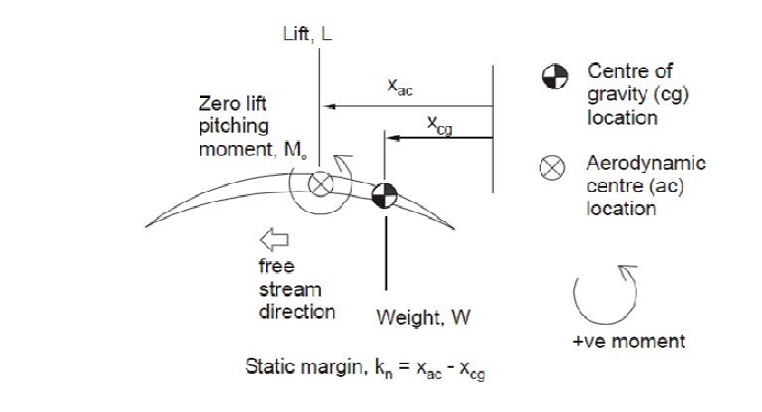
\includegraphics[width=7cm]{figures/acDiagram.png}
\caption{Aerodynamic Center}
\label{ac_center}
\end{figure}

Another assumption that was made was that initial velocity of the Frisbee is in the direction of initial pitch and roll angles. This makes sense as when throwing a Frisbee you usually release the Frisbee at the pitch and roll angles and do not apply a velocity in any other direction. Finally it was assumed that the yaw rate (or the spin rate) of the Frisbee is equal to 37 rad s\textsuperscript{-1}\cite{Lorenz2005}, and that the spin rate would remain constant throughout flight. This assumption was made based of multiple papers stating that spin rate (for a normal Frisbee flight) has a minimal effect on aerodynamic loads \cite{Pozderac2016}. Lastly, the Robins-Magnus force was neglected in this model because at low spin rates (in comparison to the translational velocity) there isn't a significant effect from the force \cite{Pozderac2016}.

\vfill
\newpage
%%%%%%%%%%%%%%%%%%%%%%%%%%%%%%%%% Mathematical Model 
\section{Mathematical Model}\label{mathModel}
The mathematical model was created using Newton's Second Law for the forces and some equations from "Simulation of a spin-stabilized sports disc" \cite{Crowther2007} for the pitching and rolling rate equations. In these calculations, three different reference frames are used. Reference frame $XYZ$ is an inertial reference frame that is stuck to the ground. Reference frame $xyz$ has axes that are always parallel to the $XYZ$, but the origin is coincident with the centroid of the Frisbee. Finally, reference frame $x'y'z'$ has an origin coincident with frame $xyz$, but rotated such that the $z'$ axis is perpendicular to the plane of the Frisbee.
\par
To account for the multiple reference frames, relative motion equations and transformation matrices were used. When moving from the global $XYZ$ reference frame to the $xyz$ reference frame, a simple translation of vectors was preformed. For example, as a part of including the wind values we had to first calculate the velocity of the Frisbee with respect to the wind for the appropriate lift and drag forces. However, for data output, the Frisbee's airspeed was converted to ground speed to ensure that the model predicted landing locations on the ground accurately. 
\par
A transformation matrix, seen on page \pageref{mathematicalDev} was used when calculating pitch and roll moments. Since calculating pitch and roll moments was much easier along the body coordinate system $x'y'z'$, the moments were calculated in that frame and transformed to the global coordinate system.
\par
This mathematical model is one of intermediate complexity. It started with the ability to take into account simple projectile motion, as well as the lift and drag forces. It also started with the assumption that center of pressure (CoP) was coincident with the center of mass (CoM) and thus calculations were quite simple. Equations \eqref{lift_vec_eq} through \eqref{eq_z_ODE} show the model that was created up to this point. Note that all calculations for this stage of the model were done in the $xyz$ coordinate system.

\begin{equation}
\vec{F}_L = \left|\vec{F}_L\right|\frac{\vec{v} \times \vec{y}'}{\left|\vec{v} \times \vec{y}'\right|} 
\label{lift_vec_eq}
\end{equation}

\begin{equation}
\vec{F}_D = -\left|\vec{F}_D\right|\frac{\vec{v}}{\left|\vec{v}\right|}
\label{drag_vec_eq}
\end{equation}

%ODE in x, equation
\begin{equation}
\centering
\ddot{x} = \frac{F_{L_{x}} + F_{D_{x}}}{m}
\label{eq_x_ODE}
\end{equation}
%ODE in y, equation
\begin{equation}
\centering
\ddot{y} = \frac{F_{L_{y}} + F_{D_{y}}}{m}
\label{eq_y_ODE}
\end{equation}
%ODE in z, equation
\begin{equation}
\centering
\ddot{z} = \frac{F_{L_{z}} + F_{D_{z}}}{m}-g
\label{eq_z_ODE}
\end{equation}

Equation \ref{lift_vec_eq} determines the lift vector by multiplying the magnitude by the unit vector of the velocity vector crossed with the body $y'$  vector. Similarly, since drag acts in the opposite direction of velocity, the drag vector is found by multiplying the magnitude of the drag force by the negative velocity unit vector in equation \eqref{drag_vec_eq}. It should be noted that even though $\dot{x}$, $\dot{y}$ and $\dot{z}$ do not appear in equations \eqref{eq_x_ODE}, \eqref{eq_y_ODE} and \eqref{eq_z_ODE}, the drag and lift forces do still depend on them. This can be seen in \eqref{eqLiftForce} and \eqref{eqDragForce} where $v$ is $\dot{x}$, $\dot{y}$ and $\dot{z}$ depending on the subscript in the forces.
\par

Then, it was decided to add complexity to the model by having the lift force and drag force act at the aerodynamic center and by removing the assumption that CoP = CoM. With the change in assumptions, the aerodynamic forces acted away from the center of mass which meant that moments were also being created. This resulted in the pitch and roll moments. The forces that act perpendicular to the plane of the Frisbee were initially calculated. Despite the change in assumption the differential equations derived above are still valid. Below in equation \eqref{body_axis_lift} shows the force of lift that is perpendicular to the plane of the Frisbee and \eqref{body_axis_drag} shows the force of drag that is perpendicular to the plane of the Frisbee.

\begin{equation}
    \vec{F}_{L_{z'}} = \vectorproj[\vec{z'}]{\vec{F}_L}
    \label{body_axis_lift}
\end{equation}

\begin{equation}
    \vec{F}_{D_{z'}} =\vectorproj[\vec{z'}]{\vec{F}_D}
    \label{body_axis_drag}
\end{equation}

\par
The direction of the aerodynamic center was found by projecting the velocity vector onto the plane of the Frisbee. Then, the precise location was found by multiplying the distance of the aerodynamic center by a unit vector. 

\begin{equation}
    \vec{ac}_{dir} = \vec{v} - \vectorproj[\vec{z'}]{\vec{v}}
    \label{ac_direction_vector}
\end{equation}

\begin{equation}
    \vec{ac}_{pos} = 0.12d \left|\vec{ac}_{dir}\right| 
    \label{ac_position_vector}
\end{equation}

The angle that the position vector of the aerodynamic center makes to the $x'$ axis is found using the scalar dot product formula. Equations \eqref{distance_to_x'} and \eqref{distance_to_y'} determine the perpendicular distance of the aerodynamic center to the $x'$ and $y'$ body axes.

\begin{equation}
    \eta = \frac{\arccos({\vec{x'} \cdot \vec{ac_{pos}}})}{\left|\vec{x'}\right| \left|\vec{ac}_{pos}\right|}
    \label{x'_angle}
\end{equation}

\begin{equation}
    d_{x'} = \sin{\eta} 
    \label{distance_to_x'}
\end{equation}

\begin{equation}
    d_{y'} = \cos{\eta} 
    \label{distance_to_y'}
\end{equation}

\begin{equation}
    P = -\left| \d_{y'}(\vec{F}_{L_{z'}} +  \vec{F}_{D_{z'}}) \right|
    \label{pitching_moment}
\end{equation}

\begin{equation}
    R = \left| \d_{x'}(\vec{F}_{L_z'} +  \vec{F}_{D_{z'}}) \right|
    \label{rolling_moment}
\end{equation}

The distances that are used in equations \eqref{pitching_moment} and \eqref{rolling_moment} are opposite of what is expected for a non-rotating body because of the gyroscopic nature of the Frisbee. The angular momentum vector of the Frisbee wants to chase the torque produced by the applied forces, so the axis precesses in a fashion that does not seem intuitive. The pitching and rolling rate equations are taken from Crowther \cite{Crowther2007}.  

\begin{equation}
    \dot{p} = \frac{2P}{I_{z}*\dot{y}}
    \label{pitch_rate_ode}
\end{equation}

\begin{equation}
    \dot{r} = \frac{2R}{I_{z}*\dot{y}}
    \label{roll_rate_ode}
\end{equation}

The system of differential equations used to model the Frisbee's path through the air are expressed in equations \eqref{eq_x_ODE}, \eqref{eq_y_ODE}, \eqref{eq_z_ODE}, \eqref{pitch_rate_ode} and \eqref{roll_rate_ode}. The ode45 function used to numerically integrate the ordinary differential equation only supports first order differential equations, so the each second order differential equation was reduced to two first order equations. This can be seen in section \ref{matlab}.

\newpage

%%%%%%%%%%%%%%%%%%%%%%%%%%%%%%% Results
\section{Results}
Due to the amount of parameters that the program can handle, this section will demonstrate the results of the program with changes in multiple parameters at a time. If the reader would like to experiment with the conditions, the repository is available at: \url{https://github.com/johnstonbrendan/202_Project}.
\par
The first result shown is a baseline result. This is what the program produces when given the most basic initial parameters. These initial parameters are:
startHeight=2m, Wind Speed=0, ThrowV=14ms\textsuperscript{-1}, r=0, p=0, spinRate=37rad s\textsuperscript{-1}
With these initial parameters the 3D plot and the individual x,y,x with respect to t plots can be seen in Figures \ref{Baseline 3D Plot}, \ref{Baseline y Plot}, \ref{Baseline x Plot} and \ref{Baseline z Plot} in section \ref{subsec::result plots}. These initial conditions are those of a flat throw and thrown by an average Frisbee thrower \cite{Morrison2005}.
\par
\par
Case 1 is one with a given initial pitch as well as a higher spin Rate and faster throw. The initial conditions that were changed from the base line and their values are: ThrowV=20ms\textsuperscript{-1}, p=10\degree , spinRate=40rad s\textsuperscript{-1}.
This model would be more accurate for a more advanced Frisbee thrower and the plots can be seen from Figures \ref{Case 1 3D Plot}, \ref{Case 1 y Plot}, \ref{Case 1 x Plot} and \ref{Case 1 z Plot} in section \ref{subsec::result plots}.
\par
Case 2 is one with a given initial pitch as well as an initial roll. The initial conditions that were changed from the base line and their values are: p=10\degree and r=10\degree. The plots generated from these changed conditions can be seen in Figure \ref{Case 2 3D Plot}, \ref{Case 2 y Plot}, \ref{Case 2 x Plot} and \ref{Case 2 z Plot} in section \ref{subsec::result plots}. Given these pitch and roll conditions, the Frisbee should be much higher than the baseline did and slowly steer to the left. This can be seen in Figure \ref{Case 2 3D Plot}.
\par
Case 3 is one with a given a wind speed and an initial roll. The initial conditions that were changed from the base line and their values are: Wind Speed = [0 1 -1]m/s and r=10\degree. The plots generated from these changed conditions can be seen in Figures \ref{Case 3 3D Plot}, \ref{Case 3 y Plot}, \ref{Case 3 x Plot} and \ref{Case 3 z Plot} in section \ref{subsec::result plots}. This case demonstrates a person throwing a Frisbee with a roll angle of 10\degree into a cross wind of 1m/s in the y direction and -1m/s in the z direction. Intuitively, one would expect the wind to steer the Frisbee left and down which can be seen in Figure \ref{Case 3 3D Plot}.
\par
Case 4 is one with a given a greater start height, wind speed, initial pitch and roll. The initial conditions that were changed from the base line are: Start Height = 20m, Wind Speed = [4 0 0] m/s, p=10\degree and r=10\degree. The plots generated from these changed conditions can be seen in Figure \ref{Case 4 3D Plot}, \ref{Case 4 y Plot}, \ref{Case 4 x Plot} and \ref{Case 4 z Plot} in section \ref{subsec::result plots}. This case demonstrates if a person were to throw a Frisbee from 20m high with wind blowing in the positive x direction.




%%%%%%%%%%%%%%%%%%%%%%%%%%%%% Conclusion
\section{Conclusion}
The overall mathematical model was the solution to the system of ODEs previously proposed in the section \ref{mathModel}. Though it was not analytically solved, numercal solutions are seen in section 5. Although the supposed model was a bit on the complex side, it was still solvable through MATLAB's ode45 function. The main limitations of this model come in it's assumptions. The assumption that the difference in location between the centre of pressure and the aerodynamic center is negligible means that an initial moment that is being created at the aerodynamic center is ignored. This initial moment potentially has trickle over effects into the solution equation and may have made the model less accurate. Although the model also does not account of any advanced aerodynamic equations it has quite a high predictive capability. Given a wind speed and direction and taking into account the angle at which the Frisbee would leave someones hand and the spin rate, the model is able to solve for the flight trajectory. These initial conditions that are set are the main factors that a normal Frisbee player would consider when making a Frisbee throw. The model itself is then able to account for the changes in angle of attack, velocity (direction and magnitude), pitch, roll, lift force and drag force in order to find the flight trajectory. These are most of the major factors that effect a Frisbee's flight and thus the model seems to be internally consistent. Additionally, there were a few factors that have assumed in the equation that may potentially allow for even more excitability in the future. Two of these factors are our mass and diameter of the Fribee. Although not tested, the model technically may be able to work for Frisbee's with a mass other than 0.175kg. This is important as not all Frisbee are designed with the same mass and this expandable feature may prove important if a real life test of this model was preformed. The same can also be said when discussing the diameter of the Frisbee, which was also taken to account in our calculations although the effect of changing it has not been tested.

%%%%%%%%%%%%%%%%%%%%%%%%%%%%% Contribution
\section{Contribution}
Research was distributed evenly among the group as everyone was required to perform their own research and to document findings in a Google Doc. When it came to creating the mathematical mode everyone worked together and discussed ideas as to how to relate the force equations with each other. Since Mistry was the most familiar with MATLAB he was responsible for writing the code while Ha and Johnston would aid Mistry in writing and reviewing the code. As Mistry and Johnston made final additions to the model, Ha became tasked with writing the report to ensure that it would be finished in time. After the model was finished, the rest of the report was split by having members work on sections that they were most familiar with. 
\end{multicols}
\newpage

%%%%%%%%%%%%%%%%%%%%%%%%%%%%%% Bibliography
\bibliography{collection}
\newpage

%%%%%%%%%%%%%%%%%%%%%%%%%%%%%% Appendix
\section{Appendix}
\subsection{MATLAB Code}\label{matlab}
\label{subsec::matlab code}
\subsubsection*{Main Code}
\label{subsubsec::main code}
\lstinputlisting{MATLAB/readableCode.m}
\newpage

\subsubsection*{Functions}
\label{subsubsec::functions}
\textbf{Lift Force}
\lstinputlisting{MATLAB/calc_lift_force.m}
\textbf{Drag Force}
\lstinputlisting{MATLAB/calc_drag_force.m}
\textbf{Velocity}
\lstinputlisting{MATLAB/velocity.m}
\textbf{Angle of Attack}
\lstinputlisting{MATLAB/alpha.m}

\newpage

%%%%%%%%%%%%%%%%%%%%%%%% Result Plots
\subsection{Results Plots}
\label{subsec::result plots}
%%%%%%%%%%%%%% Baseline Plots
%3D Plot
\subsubsection{Baseline Plots}
\begin{figure}[H]
\centering
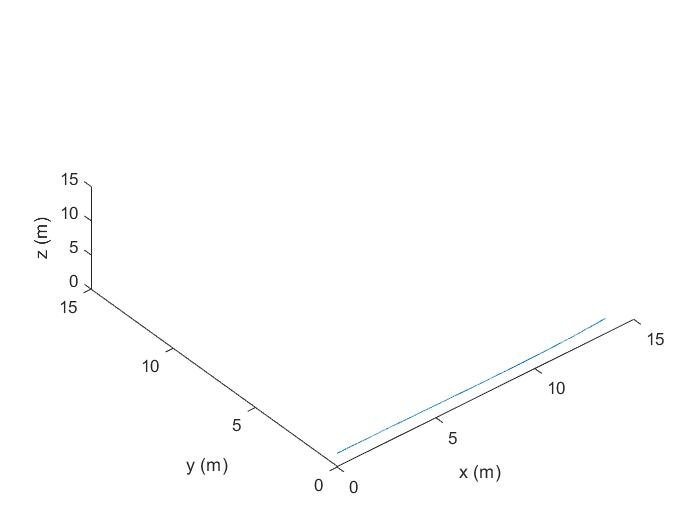
\includegraphics[width=15cm]{figures/baseline_3D.jpg}
\caption{Baseline 3D Plot}
\label{Baseline 3D Plot}
\end{figure}
\begin{multicols}{3}

%y plot
\begin{figure}[H]
\centering
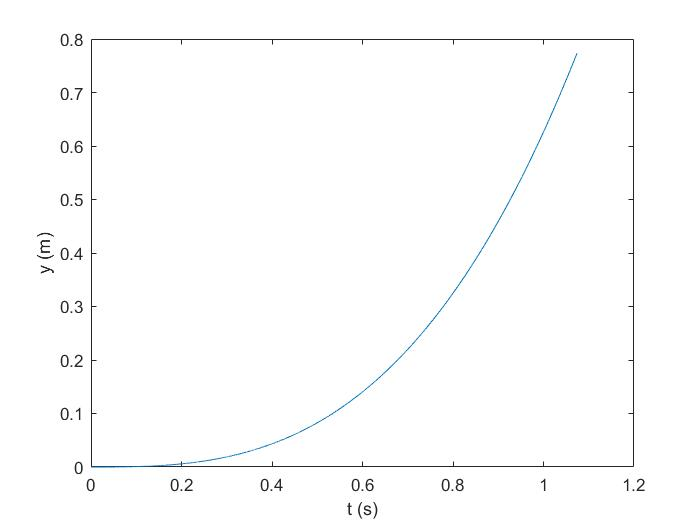
\includegraphics[width=7cm]{figures/baseline_y.jpg}
\caption{Baseline y Plot}
\label{Baseline y Plot}
\end{figure}

%x plot
\begin{figure}[H]
\centering
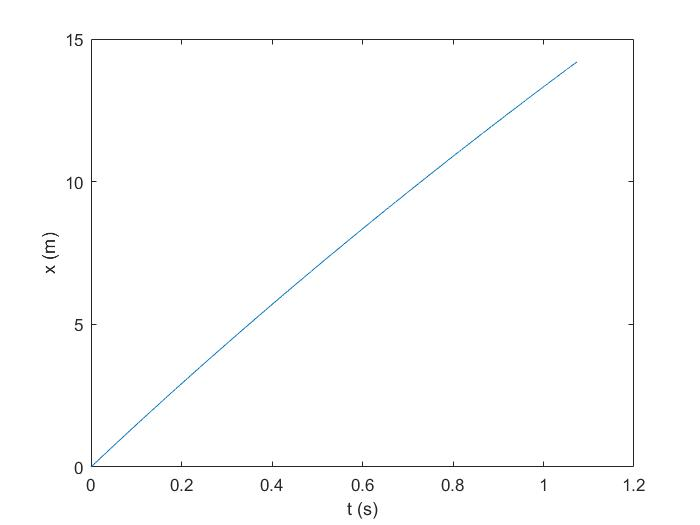
\includegraphics[width=7cm]{figures/baseline_x.jpg}
\caption{Baseline x Plot}
\label{Baseline x Plot}
\end{figure}

%z plot
\begin{figure}[H]
\centering
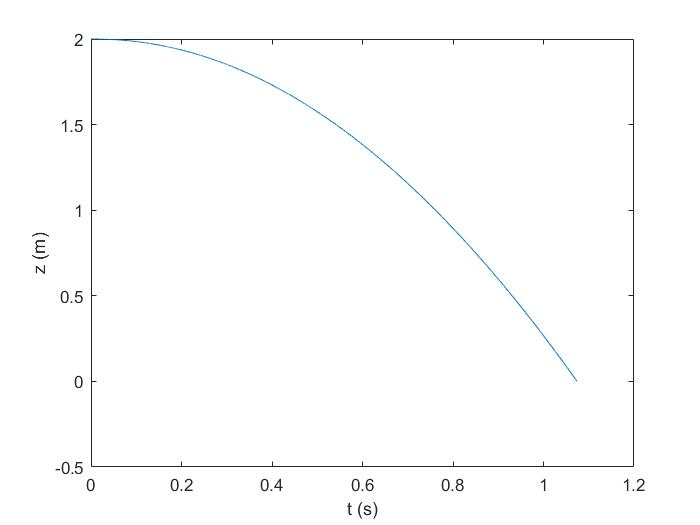
\includegraphics[width=7cm]{figures/baseline_z.jpg}
\caption{Baseline z Plot}
\label{Baseline z Plot}
\end{figure}
\end{multicols}
\newpage

%%%%%%%%% Case 1 Plots
%3D Plot
\subsubsection{Case 1 Plots}
\begin{figure}[H]
\centering
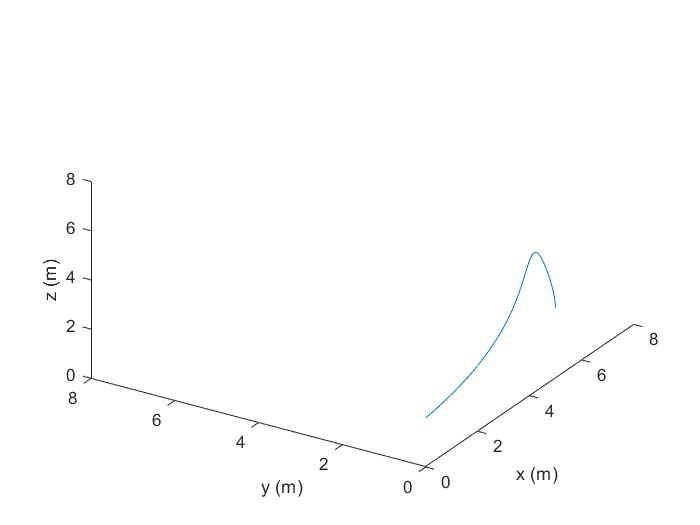
\includegraphics[width=15cm]{figures/case_1_3D.jpg}
\caption{Case 1 3D Plot}
\label{Case 1 3D Plot}
\end{figure}

\begin{multicols}{3}

%y Plot
\begin{figure}[H]
\centering
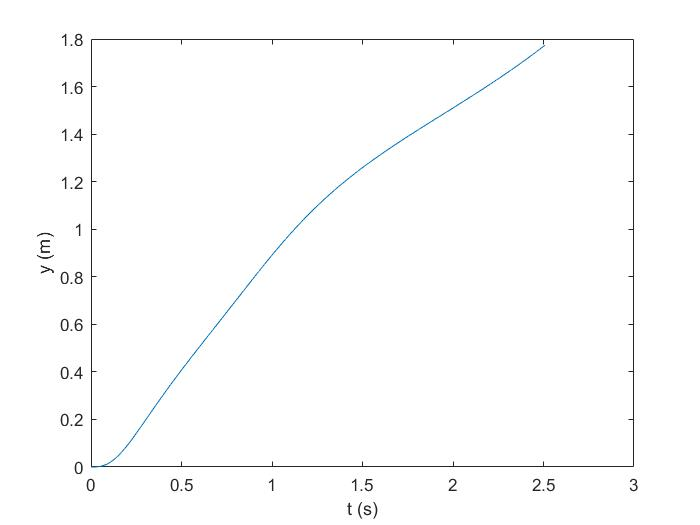
\includegraphics[width=7cm]{figures/case_1_y.jpg}
\caption{Case 1 y Plot}
\label{Case 1 y Plot}

%x plot
\end{figure}
\begin{figure}[H]
\centering
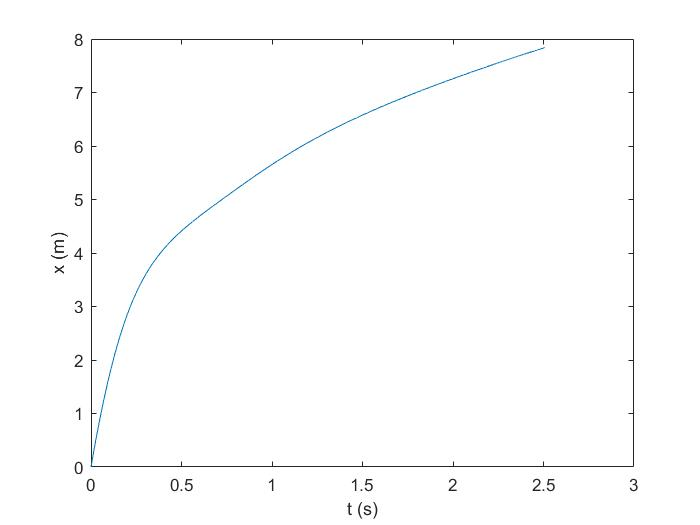
\includegraphics[width=7cm]{figures/case_1_x.jpg}
\caption{Case 1 x Plot}
\label{Case 1 x Plot}
\end{figure}
%z plot
\begin{figure}[H]
\centering
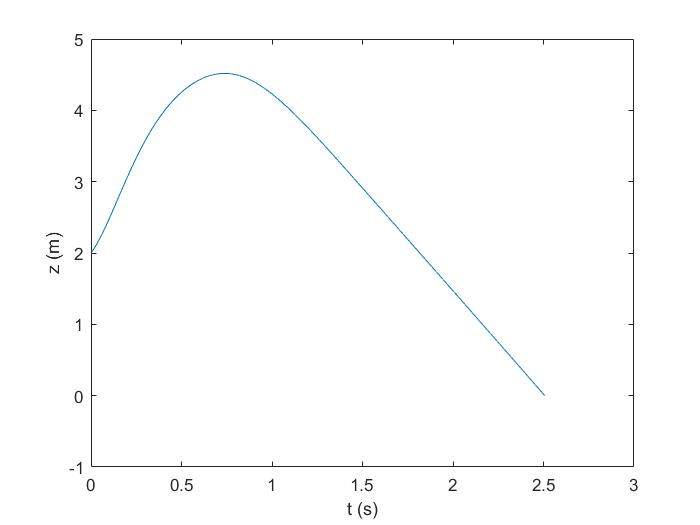
\includegraphics[width=7cm]{figures/case_1_z.jpg}
\caption{Case 1 z Plot}
\label{Case 1 z Plot}
\end{figure}

\end{multicols}
\newpage
%%%%%%%%%% Case 2 Plots
%3D Plot
\subsubsection{Case 2 Plots}
\begin{figure}[H]
\centering
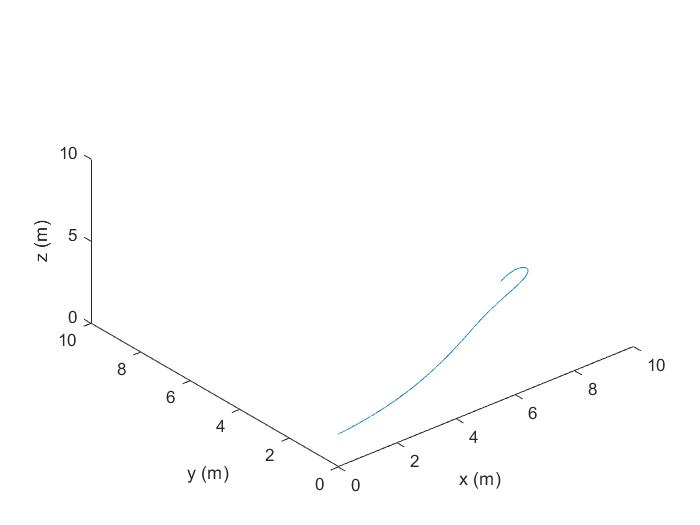
\includegraphics[width=15cm]{figures/case_2_3D.jpg}
\caption{Case 2 3D Plot}
\label{Case 2 3D Plot}
\end{figure}

\begin{multicols}{3}

%y Plot
\begin{figure}[H]
\centering
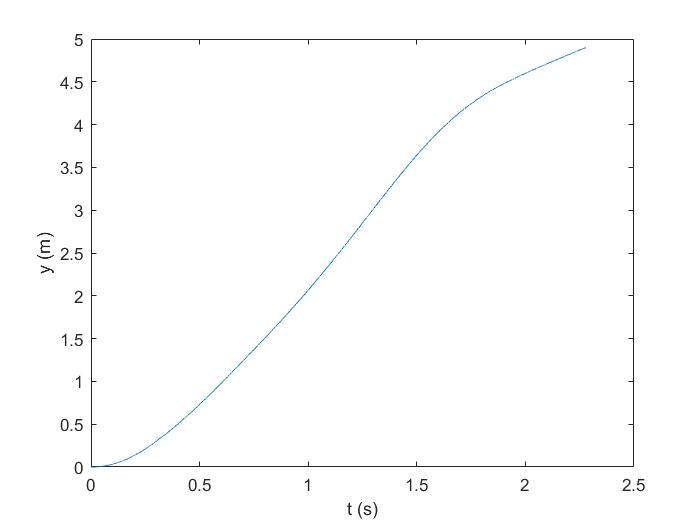
\includegraphics[width=7cm]{figures/case_2_y.jpg}
\caption{Case 2 y Plot}
\label{Case 2 y Plot}

%x plot
\end{figure}
\begin{figure}[H]
\centering
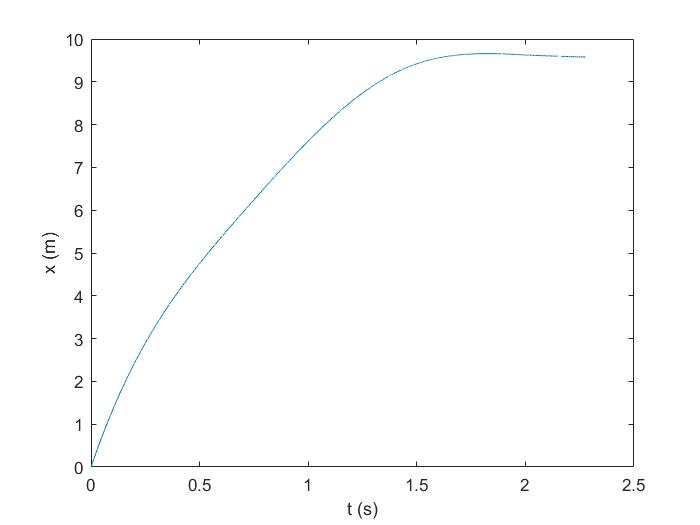
\includegraphics[width=7cm]{figures/case_2_x.jpg}
\caption{Case 2 x Plot}
\label{Case 2 x Plot}
\end{figure}
%z plot
\begin{figure}[H]
\centering
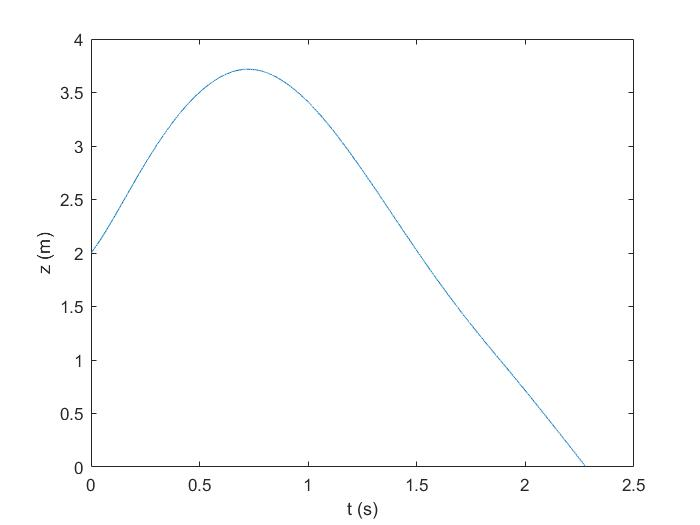
\includegraphics[width=7cm]{figures/case_2_z.jpg}
\caption{Case 2 z Plot}
\label{Case 2 z Plot}
\end{figure}

\end{multicols}
\newpage
%%%%%%%%%% Case 3 Plots
%3D Plot
\subsubsection{Case 3 Plots}
\begin{figure}[H]
\centering
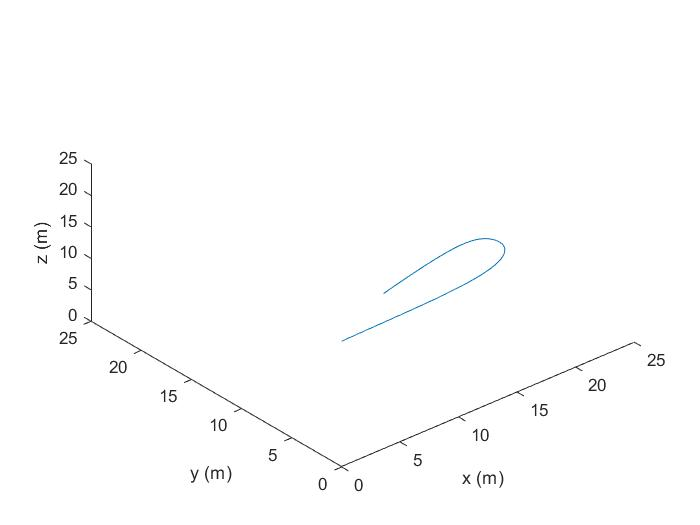
\includegraphics[width=15cm]{figures/case_3_3D.jpg}
\caption{Case 3 3D Plot}
\label{Case 3 3D Plot}
\end{figure}

\begin{multicols}{3}

%y Plot
\begin{figure}[H]
\centering
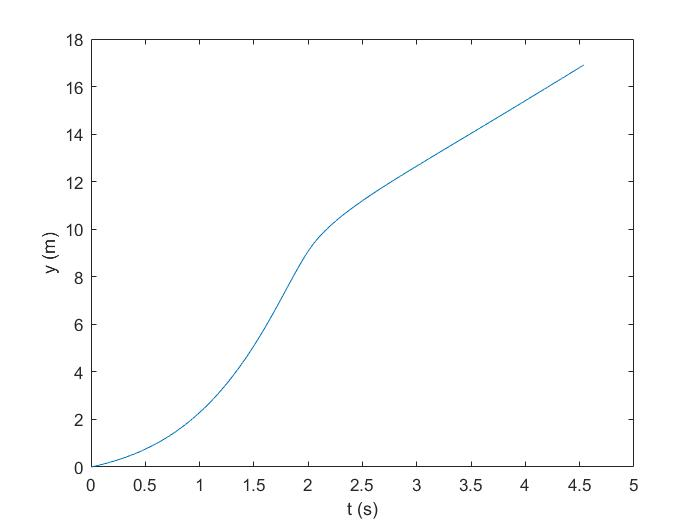
\includegraphics[width=7cm]{figures/case_3_y.jpg}
\caption{Case 3 y Plot}
\label{Case 3 y Plot}

%x plot
\end{figure}
\begin{figure}[H]
\centering
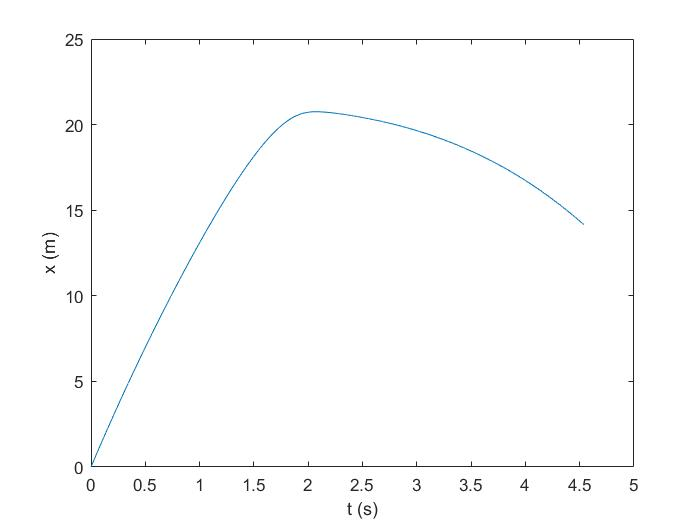
\includegraphics[width=7cm]{figures/case_3_x.jpg}
\caption{Case 3 x Plot}
\label{Case 3 x Plot}
\end{figure}
%z plot
\begin{figure}[H]
\centering
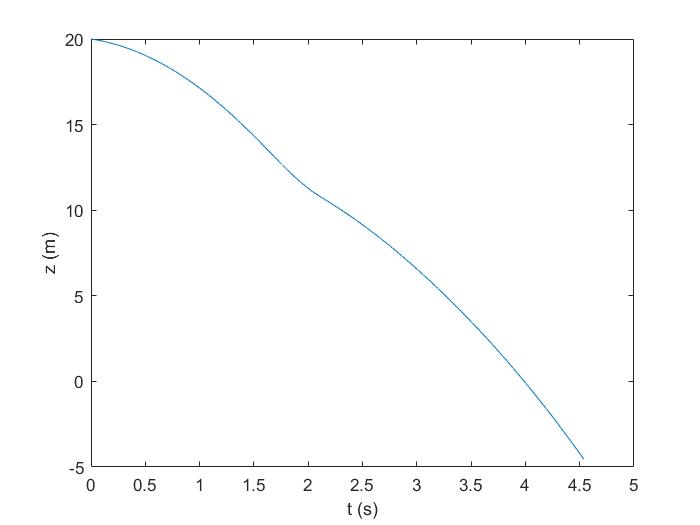
\includegraphics[width=7cm]{figures/case_3_z.jpg}
\caption{Case 3 z Plot}
\label{Case 3 z Plot}
\end{figure}

\end{multicols}
\newpage
%%%%%%%%%% Case 4 Plots
%3D Plot
\subsubsection{Case 4 Plots}
\begin{figure}[H]
\centering
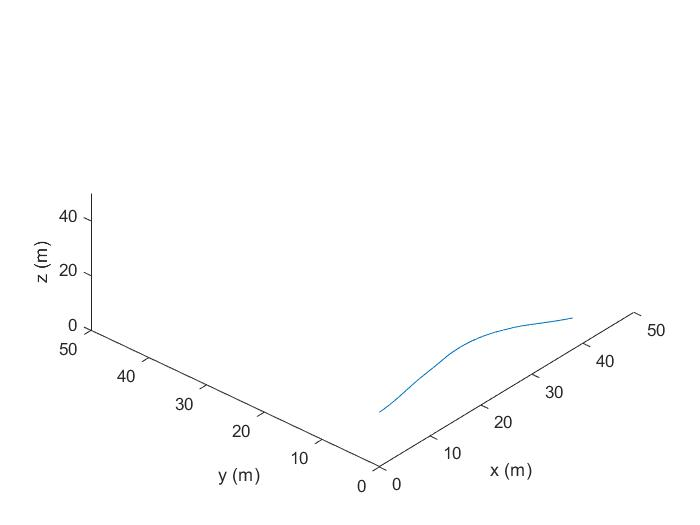
\includegraphics[width=15cm]{figures/case_4_3D.jpg}
\caption{Case 4 3D Plot}
\label{Case 4 3D Plot}
\end{figure}

\begin{multicols}{3}

%y Plot
\begin{figure}[H]
\centering
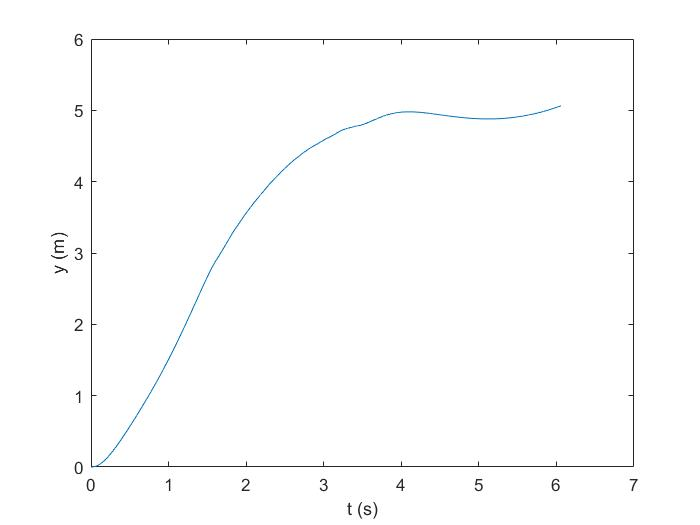
\includegraphics[width=7cm]{figures/case_4_y.jpg}
\caption{Case 4 y Plot}
\label{Case 4 y Plot}

%x plot
\end{figure}
\begin{figure}[H]
\centering
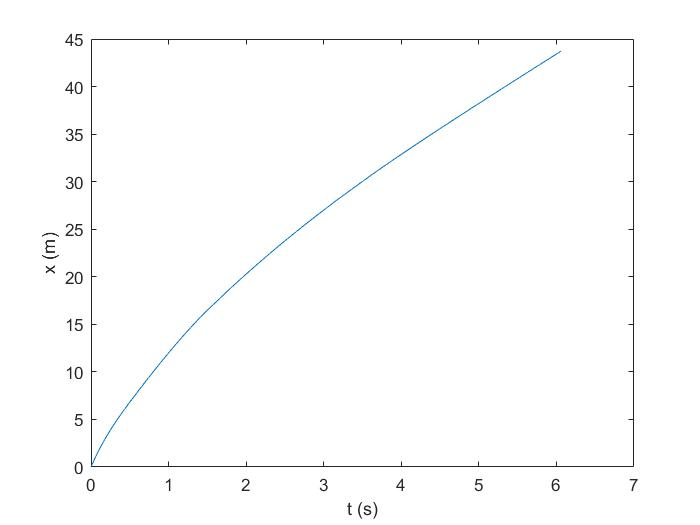
\includegraphics[width=7cm]{figures/case_4_x.jpg}
\caption{Case 4 x Plot}
\label{Case 4 x Plot}
\end{figure}
%z plot
\begin{figure}[H]
\centering
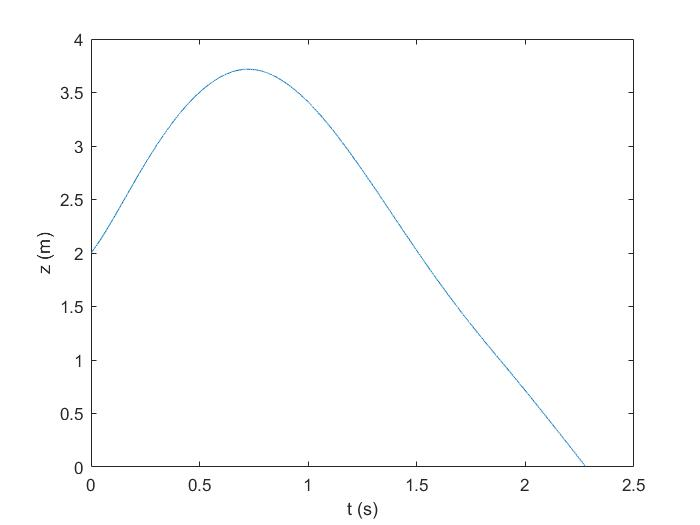
\includegraphics[width=7cm]{figures/case_2_z.jpg}
\caption{Case 4 z Plot}
\label{Case 4 z Plot}
\end{figure}

\end{multicols}
%%%%%%%%%%%%%%%%%%%%%%%%%%%%%%%% Mathematical Development
\subsection{Mathematical Development} \label{mathematicalDev}
This is the transformation matrix used to convert the $xyz$ frame to the $XYZ$ frame: 
\begin{equation}
T = 
\begin{bmatrix}
1 && 0 && 0 \\ 
0 && \cos{\phi} && -\sin{\phi} \\
0 && sin{\phi} && cos{\phi}
\end{bmatrix}
\begin{bmatrix}
\cos{\theta} && 0 && \sin{\theta} \\ 
0 && 1 && 0 \\
-\sin{\theta} && 0 && \cos{\theta}\\
\end{bmatrix}
\end{equation}
where $\phi$ is the roll angle and $\theta$ is the pitch angle. 

\end{document}
%%% Local Variables: 
%%% mode: latex
%%% TeX-master: t
%%% End: 
